\section{Программное обеспечение для решения поставленной задачи}

\subsection{Описание программы}

\subsubsection{Общие сведения}
Требования настоящего руководства применяются при:

\begin{itemize}
\item опытной эксплуатации
\item приемочных испытаниях
\item промышленной эксплуатации
\item предварительных комплексных испытаниях
\end{itemize}

Чтобы использовать данную программу необходимо понимать предметную область. А именно понимать, как физически устроен процесс горячей прокатки. Такими знаниями обычно обладают операторы оборудования, управляющие процессом. Тем не менее, необходимым уровенем знаний обладают не только люди этой профессии и, при должном уровне доступа к этой программе, могут пользоваться и другие.

\subsubsection{Функциональное назначение}
Программа может при помощи решения дифференициальных уравнений теплопроводности в частных производных рассчитывать температурное распределение в полосе и рабочем слое валка. Для более точного расчета используются физические законы, описывающие энергосиловые характеристики процесса, с помощью которых программа рассчитывает тепловое распределение более точно. Вся полученная информация выводится в понятных интерактивных графиках для наглядного отображения получившихся параметров горячей прокатки.

Программный продукт применяется для расчета основных характеристик при работе с процессом горячей прокатки. Получаемые данные необходимы для оценки изношенности рабочих валков, а так же для оценки уровня нагрева рабочего слоя. Информация о нагреве нужна для оптимизации процесса охлаждения валка.

\subsubsection{Описание логической структуры}

Программный продукт был реализован на языке C++ при помощи кроссплатфоремнного фреймворка Qt \cite{QT}. Qt позволяет запускать написанное с его помощью программное обеспечение в большинстве современных операционных систем путём простой компиляции программы для каждой системы без изменения исходного кода. Включает в себя все основные классы, которые могут потребоваться при разработке прикладного программного обеспечения, начиная от элементов графического интерфейса и заканчивая классами для работы с сетью, базами данных и XML. Является полностью объектно-ориентированным, расширяемым и поддерживающим технику компонентного программирования.

Qt создала себе репутацию средства разработки межплатформенных приложений, но благодаря своему интуитивному и мощному программному интерфейсу во многих организациях Qt используется для одноплатформенных разработок.

В основном расчете используются классы описанные ниже. В программе фигурируют и другие классы, но они нужны для вывода информации и других дополнительных функций.

1) \textbf{Roll} - класс для описания валка.

Содержит в себе физические свойства металла валка. А именно теплоемкость - с, плотность материала - rho, теплопроводность - lambda, радиус валка - radius,  толщина рабочего слоя валка - mmToHeat и скорость вращения - speed.

В этом классе представлены методы для получения значений, описанных выше.
\begin{itemize}
\item[•] double getR() - возвращает радиус валка;
\item[•] double getC() - возвращает теплоемкость валка;
\item[•] double getRho() - возвращает плотность металла валка;
\item[•] double getLambda() - возвращает теплопроводность валка;
\item[•] double getSpeed() - возвращает скорость вращения валка в м/с;
\item[•] double countmmToHeat() - возвращает толщину рабочего слоя валка.
\end{itemize}

А так же представлена функция возвращающая распределение температуры в глубину в валке на входе в очаг - double initT(double r) и функция, задающая это распределение double setInitT(QVector<double> t).

2) \textbf{Scale} - класс для описания окалины, образующуюся на полосе во время ее проката.

Содержит в себе физические свойства окалины: теплопроводность - lambda и ее толщину - thickness.

В этом классе нет методов.

3) \textbf{Strip} - класс для описания прокатной полосы.

Содержит в себе физические свойства металла полосы. А именно теплоемкость - с, плотность материала - rho, теплопроводность - lambda.

В этом классе представлены методы для получения значений, описанных выше.
\begin{itemize}
\item[•] double getC() - возвращает теплоемкость полосы;
\item[•] double getRho() - возвращает плотность металла полосы;
\item[•] double getLambda() - возвращает теплопроводность полосы.
\end{itemize}

А так же представлена функция возвращающая распределение температуры в глубину в полосе на входе в очаг - double initT(double r).

4) \textbf{Focus} - класс, в котором собираются физические объекты для описания очага деформации.

Содержит в себе все параметры очага деформации. В первую очередь в этот класс входят валок - roll, полоса - strip, участвующие в процессе и окалина - scale, которая образуется при этом процессе. Дополнительно для описания особенностей очага представлены следующие поля:
\begin{itemize}
\item[•] h\_b - толщина полосы на входе в очаг;
\item[•] h\_a - толщина полосы на выходе из очага;
\item[•] length - длина очага;
\item[•] phi\_max - правая граница области очага для угла;
\item[•] r\_max - максимальное значение радиуса в области очага;
\item[•] alpha - величина угла во второй части очага (см. рис. \ref{4});
\item[•] beta - величина угла в первой части очага (см. рис. \ref{4}).
\end{itemize}

В этом классе представлены следующие методы:
\begin{itemize}
\item[•] Roll getRoll() - возращает валок, участвующий в процессе прокатки в данном очаге;
\item[•] Strip getStrip() - возращает полосу, участвующую в процессе прокатки в данном очаге;
\item[•] Scale getScale() - возращает окалину, получившуюся в процессе прокатки в данном очаге;
\item[•] double getHBefore() - возращает толщину полосы на входе в очаг;
\item[•] double getHAfter() - возращает толщину полосы на выходе из очага;
\item[•] double maxR(double phi) - возращает правую границу для радиуса в текущем слое. Принимает значения угла в интересующем слое;
\item[•] double epsH(double h, double h\_max) - возращает относительное обжатие полосы. Принимает толщину полосы в 2 состояниях. Можно использовать как для узнавания обжатия на соседних слоях, так и на всем очаге;
\item[•] double curH(double phi) - возращает толщину полосы на текущем слое.
\end{itemize}

5) \textbf{diffEquation} - класс для решения дифференциального уравнения теплопроводности в частных производных при заданных параметрах горячей прокатки.

Содержит в себе все параметры для численного решения уравнения. Данные очага берутся из объекта focus класса Focus, а для расчета используются следующие поля:
\begin{itemize}
\item[•] u - матрица значений температуры в узлах разностной сетки;
\item[•] h - шаг по радиусу;
\item[•] theta - шаг по углу;
\item[•] M - количество точек по радиусу;
\item[•] N - количество точек по углу;
\item[•] NBack - точка ограничивающая зону отставания (см. рис. \ref{5});
\item[•] NForward - точка ограничивающая зону опережения (см. рис. \ref{5});
\item[•] Nneutr - точка в зоне прилипания, где скорость проката полосы и скорость вращения валка совпадают (см. рис. \ref{5});
\item[•] tauContAbs - касательное напряжение;
\item[•] tauShear - предел текучести.
\end{itemize}

В этом классе представлены следующие методы:
\begin{itemize}
\item[•] void solveFocus() - функция для решения уравнения теплопроводности в очаге деформации;
\item[•] void solveNonFocus(double t) - функция для решения уравнения теплопроводности вне очага деформации, принимает температуру воды или воздуха, которым охлаждается валок;
\item[•] Focus getFocus() - возвращает объект очага деформации;
\item[•] int MUpdate(double angle, double rstep) - возвращает количество точек по радиусу для расчета в очередном слое. Принимает значение угла в очередном слое и шаг по радиусу;
\item[•] double q(int i) - возвращает величину теплового потока в \textit{i}-том слое;
\item[•] double f(int i, int j) - возвращает величину приращения температуры от предыдущего слоя в точке с координатами (\textit{i, j}) в разностной сетке;
\item[•] double Kdef(double phi) - возвращает величину сопротивления деформации на определнном слое. Принимает значение угла в нужном слое.
\end{itemize}

\newpage

\blockschema{16}{Диаграмма классов}

\subsubsection{Используемые технические средства}
Минимальная конфигурация технических и общесистемных программных средств должна соответствовать следующим параметрам:

\begin{itemize}
\item процессор с тактовой частотой не ниже 1 ГГц;
\item ОЗУ не менее 512 Мбайт;
\item свободное дисковое пространство 40.7 Мбайт;
\item монитор с разрешением $1280\times 800$ и больше;
\item клавиатура;
\item мышь;
\item установленный Microsoft Visual C++ 2008 Redistributable или моложе;
\item ОС MS Windows XP SP2 (32 bit version) или моложе.
\end{itemize}

Так же для работы в папке с программой должны находиться следующие библиотеки:
\begin{itemize}
\item libgcc\_s\_dw2-1.dll;
\item libstdc++-6.dll;
\item libwinpthread-1.dll;
\item Qt5Core.dll;
\item Qt5Gui.dll;
\item Qt5PrintSupport.dll;
\item Qt5Widgets.dll;
\item platforms/qwindows.dll.
\item platforms/qwindowsd.dll.
\end{itemize}

\subsubsection{Установка и удаление}
Для установки ПО необходимо перенести с носителя дистрибутива исполняемый файл и файлы библиотек, лежащие с ним в одной папке, в папку на своем компьютере.

Для удаления ПО необходимо удалить исполняемый файл и файлы библиотек, лежащие с ним в одной папке со своего компьютера.

\subsubsection{Вызов и загрузка}
Перед началом работы пользователю нужно сделать следующее:
\begin{enumerate}
\item Зайти в папку, в которой лежит программа.
\item Запустить двойным щелчком программу <<heat.exe>>.
\item После появления главного окна программы можно начинать работу.
\blockschema{7}{Главное окно программы}

\end{enumerate}

\subsubsection{Входные данные}
\begin{itemize}
\item Параметры металла: физические параметры металлов полосы и валка (коэффициент теплопроводности, плотность материалов и теплоемкость).
\item Общие настройки: радиус валка, скорость его вращения, глубина валка, на которую будет рассчитываться распространение тепла, время моделирования и параметры дискретизации (количество точек по радиусу и по кругу вращения валка).
\item Параметры очага деформации: толщина полосы на входе в очаг и толщина полосы на выходе из очага.
\item Параметры охлаждения валка: температуры воздуха и воды, которыми охлаждается валок.
\end{itemize}

\subsubsection{Выходные данные}
На выходе пользователь получает графики распределения энергосиловых характеристик на протяжении всей длины очага деформации а таблицу со значениями температуры во всех узлах дискретизации.

\subsection{Руководство пользователя}
\subsubsection{Назначение программы}
Программа может при помощи решения дифференициальных уравнений теплопроводности в частных производных рассчитывать температурное распределение в полосе и рабочем слое валка. Для более точного расчета используются физические законы, описывающие энергосиловые характеристики процесса, с помощью которых программа рассчитывает тепловое распределение более точно. Вся полученная информация выводится в понятных интерактивных графиках для наглядного отображения получившихся параметров горячей прокатки.

Программный продукт применяется для расчета основных характеристик при работе с процессом горячей прокатки. Получаемые данные необходимы для оценки изношенности рабочих валков, а так же для оценки уровня нагрева рабочего слоя. Информация о нагреве нужна для оптимизации процесса охлаждения валка.

\subsubsection{Условия выполнения программы}
Для полноценной работы программы необходимы следующие системные требования:

\begin{itemize}
\item процессор с тактовой частотой не ниже 1 ГГц;
\item ОЗУ не менее 512 Мбайт;
\item свободное дисковое пространство 40.7 Мбайт;
\item монитор с разрешением $1280\times 800$ и больше;
\item клавиатура;
\item мышь;
\item установленный Microsoft Visual C++ 2008 Redistributable или моложе;
\item ОС MS Windows XP SP2 (32 bit version) или моложе.
\end{itemize}

Так же для работы в папке с программой должны находиться следующие библиотеки:
\begin{itemize}
\item libgcc\_s\_dw2-1.dll;
\item libstdc++-6.dll;
\item libwinpthread-1.dll;
\item Qt5Core.dll;
\item Qt5Gui.dll;
\item Qt5PrintSupport.dll;
\item Qt5Widgets.dll;
\item platforms/qwindows.dll.
\item platforms/qwindowsd.dll.
\end{itemize}
\subsubsection{Выполнение программы}
%\newpage
\begin{longtable}{|p{3cm}|p{4cm}|p{8cm}|}
\hline
Функции & Задачи & Описание\\
\hline
Задание входных данных для расчета всех характеристик & Настройка вручную & Перед началом работы необходимо убедиться, что настройки оборудования соответствуют значениям, введенным в программе для расчета необходимых величин. В настройках задаются все параметры, указанные в п. 3.1.7. Все настройки сохраняются в файл для дальнейшего их чтения. Сохранение настроек в файл позволяет удобно переносить с одного носителя на другой.\\ \cline{2-3}
%\hline
 & Загрузка из файла & Параметры можно переносить с одного устройство на другое, а так же использовать преднастройки, чтобы не тратить время на ввод данных. Делается это путем загрузки из нужного файла.\\
\hline
Основной расчет & Расчет всех необходимых характеристик процесса горячей прокатки & Основная функция программы. Производит расчет с заданными параметрами, считанными из файла настроек (см. Настройка параметров). В виде результата выводится таблица с распределением температур. Для анализа результатов выодятся графики энергосиловых характеристик и график распределения температуры на выходе из очага деформации в полосе и в рабочем слое валка.\\
\hline
\end{longtable}

1) Настройка параметров вручную.

Для выполнения этой функции необходимо выполнить следующие действия: на главном экране нажать на кнопку <<Параметры>>.
\blockschema{11}{Кнопка для открытия окна с настройками}

Появится дополнительное окно, в котором необходимо указать параметры, описанные в п. 3.1.7.
\fig{8}{Окно настроек}

После ввода данных нужно нажать на кнопку <<Сохранить и применить параметры>>.

2) Загрузка параметров из файла.

Для выполнения этой функции необходимо в окне параметров нажать на кнопку <<Загрузить параметры из файла>> или на главном окне в меню <<Файл>> выбрать пункт <<Загрузить параметры>>.

\begin{figure}[h] 
\label{21} 
\begin{minipage}[h]{0.49\linewidth} 
\center{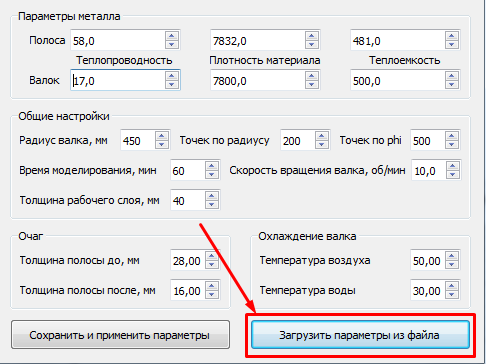
\includegraphics[width=0.9\linewidth]{20} \\} 
\end{minipage} 
\hfill 
\begin{minipage}[h]{0.49\linewidth} 
\center{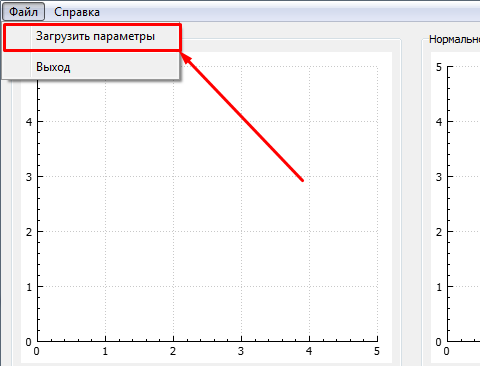
\includegraphics[width=0.9\linewidth]{21} \\ } 
\end{minipage} 
\caption{Кнопка для открытия окна с настройками} 
\end{figure}

Затем выбрать файл формата <<.hrp>>. Настройки автоматически сохранятся, соответственно дополнительно нажимать на кнопку <<Сохранить и применить параметры>> не нужно.

3) Основной расчет.

Чтобы выполнить эту функцию необходимо на главном экране нажать на кнопку <<Рассчитать температуру>>.
\blockschema{12}{Кнопка для основного расчета}

В течение нескольких секунд будет производиться расчет и вывод полученной информации на экран. Необходимо немного подождать завершения операции. В результате на экране появятся графики изменения самых важных величин (теплового потока, нормального и касательного напряжений, предела текучести и сопротивления деформации) по длине очага и график распределения тепла на выходе из очага. И, что самое главное, разностную сетку со значениями температуры в рабочем слое валка и в полосе.
\blockschema{15}{Главное окно после расчетов}

\subsubsection{Сообщения оператору}
В случае возникновения ошибок при работе с программой, не описанных ниже в данном разделе, необходимо обращаться к ответственному администратору.

\begin{itemize}
\item <<Настройки не загружены!>>
\fig{14}{Ошибка заполнения полей}
\end{itemize}

Такая ошибка может возникнуть из-за импорта настроек из файла с нарушенной структурой, либо с недостающими параметрами. Так же она может возникнуть из-за ошибочного ввода данных. Для исправления необходимо сохранить нужные параметры заново так, как описано в п. 3.2.3.

В качестве контрольного примера рекомендуется выполнить операции, описанные в п. 3.2.3. настоящего документа.

\newpage